% =====================================================================
%  CDA / Gemini letter -- Section 2.2 contribution (T. Bulmus)
%
%  SELF-CONTAINED. Upload this ONE file to Overleaf, set it as the main
%  document, hit Recompile. Nothing else is needed -- no \input, no
%  extra files, no aa.cls.
%
%  It is set as a two-column article purely so that figure* behaves the
%  way it will in A&A. The two placeholder sections exist only to make
%  the cross-references resolve and to show where the new subsection
%  slots in; delete them when transplanting into the real paper.
% =====================================================================
\documentclass[twocolumn,a4paper,10pt]{article}

\usepackage[margin=20mm]{geometry}
\usepackage[T1]{fontenc}
\usepackage{amsmath}
\usepackage{graphicx}        % \resizebox -- tikz does NOT reliably provide this
\usepackage{tikz}
\usetikzlibrary{arrows.meta,positioning,calc}

\begin{document}

\section{Methods}
\label{sec:methods}

\subsection{Pre-processing and few-shot classification}
\label{sec:classification}

\textit{[Placeholder for the existing Sect.~2.1 text -- rendering of the
spectra, the plotting conventions, and the few-shot classification setup.
Delete this subsection when transplanting.]}

% =====================================================================
%  >>>>>>>>>>  THE CONTRIBUTION STARTS HERE  <<<<<<<<<<
% =====================================================================

\subsection{Agentic construction and two-stage neuro-symbolic adjudication}
\label{sec:agentic}

The classifier described in Sect.~\ref{sec:classification} was not hand-tuned.
Both the system instruction, the contrastive few-shot reference set, and the
two-stage inference and adjudication pipeline were produced by a multi-agent
system built on the Google Agent Development Kit (ADK), in which a
deterministic orchestrator chains a set of specialised sub-agents, each
responsible for one reproducible step of the experiment
(Fig.~\ref{fig:agentworkflow}). The implementation is publicly available at
\texttt{github.com/turanbulmus/cda-dust-analyzer}.

% =====================================================================
%  Figure: agent architecture, spanning both columns.
%  Absolute coordinates in mm -- no relative chains, so a change in one
%  box cannot cascade the rest out of place.
% =====================================================================
\begin{figure*}[t]
\centering
\resizebox{\textwidth}{!}{%
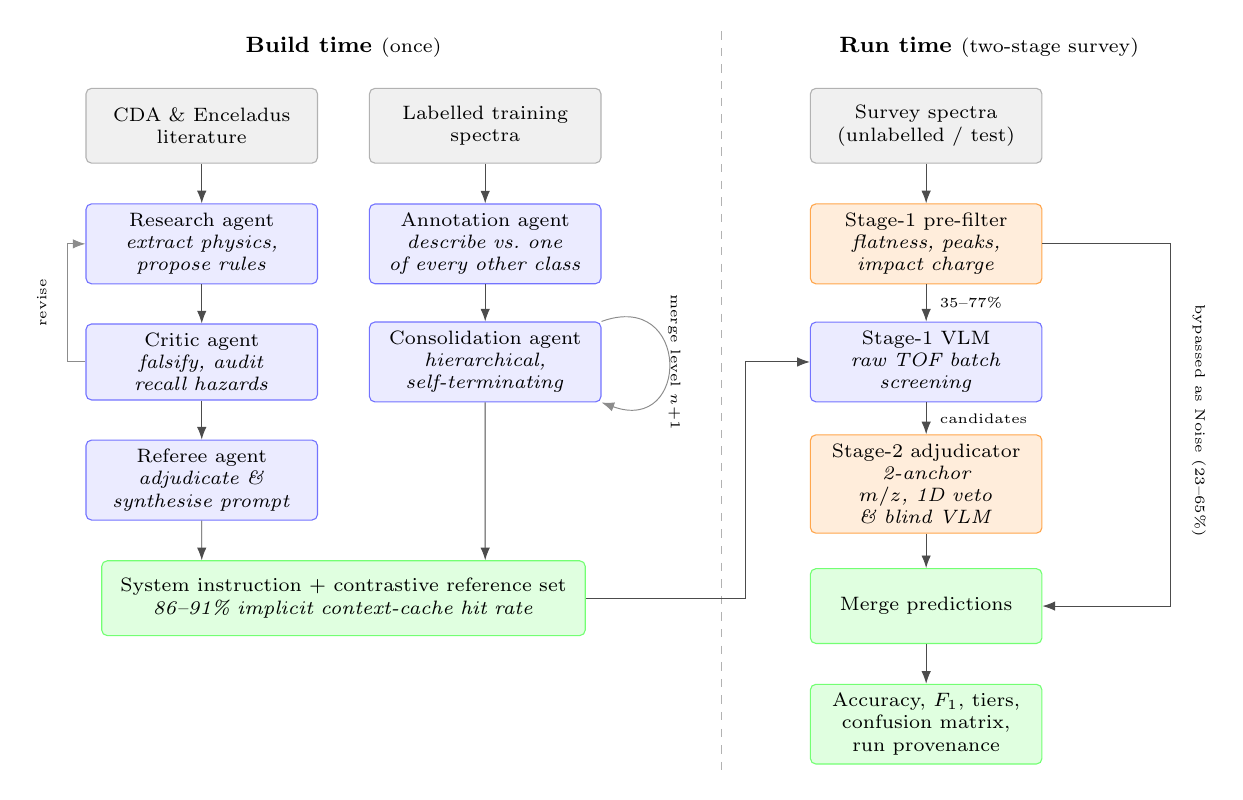
\begin{tikzpicture}[
  x=1mm, y=1mm,
  font=\scriptsize,
  box/.style   = {draw, rounded corners=2pt, align=center,
                  minimum height=9.5mm, text width=28mm, inner xsep=2pt},
  agent/.style = {box, fill=blue!8,    draw=blue!55},
  data/.style  = {box, fill=gray!12,   draw=gray!60},
  gate/.style   = {box, fill=orange!14, draw=orange!70},
  outbox/.style = {box, fill=green!12,  draw=green!55},
  ttl/.style    = {font=\footnotesize\bfseries},
  ar/.style     = {-{Latex[length=1.6mm]}, draw=black!70, line width=0.35pt},
  fb/.style     = {ar, draw=black!45},
]

% ---------- panel separator (drawn first, so arrows sit on top) ----------
\draw[dashed, draw=black!30] (86,6) -- (86,-88);

\node[ttl] at (38,4)  {Build time \textnormal{\scriptsize (once)}};
\node[ttl] at (120,4) {Run time \textnormal{\scriptsize (two-stage survey)}};

% ============ BUILD TIME : column 1 -- literature grounding =============
\node[data,  at={(20,-6)}]  (papers)   {CDA \& Enceladus\\literature};
\node[agent, at={(20,-21)}] (research) {Research agent\\\textit{extract physics,}\\\textit{propose rules}};
\node[agent, at={(20,-36)}] (critic)   {Critic agent\\\textit{falsify, audit}\\\textit{recall hazards}};
\node[agent, at={(20,-51)}] (referee)  {Referee agent\\\textit{adjudicate \&}\\\textit{synthesise prompt}};

\draw[ar] (papers)   -- (research);
\draw[ar] (research) -- (critic);
\draw[ar] (critic)   -- (referee);
\draw[fb] (critic.west) -- (3,-36) -- (3,-21) -- (research.west);
\node[font=\tiny, rotate=90, anchor=south] at (1.5,-28.5) {revise};

% ============ BUILD TIME : column 2 -- contrastive few-shot =============
\node[data,  at={(56,-6)}]  (train)  {Labelled training\\spectra};
\node[agent, at={(56,-21)}] (annot)  {Annotation agent\\\textit{describe vs.\ one}\\\textit{of every other class}};
\node[agent, at={(56,-36)}] (consol) {Consolidation agent\\\textit{hierarchical,}\\\textit{self-terminating}};

\draw[ar] (train) -- (annot);
\draw[ar] (annot) -- (consol);
\draw[fb] (consol.north east) to[out=20,in=-20,looseness=3] (consol.south east);
\node[font=\tiny, rotate=-90, anchor=south] at (78,-36) {merge level $n{+}1$};

% ============ BUILD TIME : shared artefact bundle =======================
\node[outbox, at={(38,-66)}, text width=60mm] (bundle)
      {System instruction $+$ contrastive reference set\\
       \textit{86--91\% implicit context-cache hit rate}};

\draw[ar] (referee.south) -- ([xshift=-18mm]bundle.north);
\draw[ar] (consol.south)  -- ([xshift=18mm]bundle.north);

% ============ RUN TIME : column 3 -- inference & Stage-2 ================
\node[data,   at={(112,-6)}]  (survey)  {Survey spectra\\(unlabelled / test)};
\node[gate,   at={(112,-21)}] (prefilt) {Stage-1 pre-filter\\\textit{flatness, peaks,}\\\textit{impact charge}};
\node[agent,  at={(112,-36)}] (vlm)     {Stage-1 VLM\\\textit{raw TOF batch}\\\textit{screening}};
\node[gate,   at={(112,-51.5)}] (stage2)  {Stage-2 adjudicator\\\textit{2-anchor $m/z$, 1D veto}\\\textit{\& blind VLM}};
\node[outbox, at={(112,-67)}] (merge)   {Merge predictions};
\node[outbox, at={(112,-82)}] (metrics) {Accuracy, $F_1$, tiers,\\confusion matrix,\\run provenance};

\draw[ar] (survey)  -- (prefilt);
\draw[ar] (prefilt) -- node[right, font=\tiny, xshift=0.5mm] {$35\text{--}77\%$} (vlm);
\draw[ar] (vlm)     -- node[right, font=\tiny, xshift=0.5mm] {candidates} (stage2);
\draw[ar] (stage2)  -- (merge);
\draw[ar] (merge)   -- (metrics);

% bypass route, kept in the empty fourth column so it crosses nothing
\draw[ar] (prefilt.east) -- (143,-21) -- (143,-67) -- (merge.east);
\node[font=\tiny, rotate=-90, anchor=south] at (144.5,-43.5)
      {bypassed as Noise ($23\text{--}65\%$)};

% ============ cross-panel coupling ======================================
\draw[ar] (bundle.east) -- (89,-66) -- (89,-36) -- (vlm.west);

\end{tikzpicture}%
}
\caption{Two-stage agentic workflow used to build, run, and adjudicate the
classifier. At build time (left), a three-agent loop (Research $\rightarrow$
Critic $\rightarrow$ Referee) derives and falsifies physical decision rules from
the published CDA literature, while in parallel reference spectra are annotated
contrastively and consolidated into canonical class patterns. At run time
(right), a deterministic Stage-1 pre-filter bypasses obvious noise ($23\text{--}65\%$)
before Stage-1 Gemini VLM batch screening on raw time-of-flight plots. Positive
salt-subtype candidates (\texttt{3-OH}, \texttt{3-P}) are then routed to the
Stage-2 specialist adjudicator, which performs two-anchor mass calibration
$(\hat{t}_0, \hat{a})$ on $\text{Na}^+$ ($23\,\text{u}$) and
$\text{Na}^+(\text{NaOH})$ ($63\,\text{u}$), renders dual-panel mass-calibrated
plots ($10\text{--}200\,\text{u}$ and $70\text{--}195\,\text{u}$), and applies
1D mass-window physics vetoes alongside a leak-free blind specialist VLM before
merging predictions and logging provenance.}
\label{fig:agentworkflow}
\end{figure*}

\paragraph{Literature grounding.}
The system instruction was not written from the instrument description alone.
A research agent ingested the full text of the key CDA and Enceladus
publications and was tasked with extracting the physical and chemical
constraints that bear on classification --- the mass resolution of
$m/\Delta m \approx 10$--$50$, the $t = t_0 + a\sqrt{m/z}$ time-of-flight
mapping ($a \approx 0.473\,\mu\text{s}$) and the resulting trigger shift of up
to $\pm 50$ channels, the hydronium cluster combs of icy grains, the Mg-rich
and Fe-depleted silicate cations, the $12$--$13$\,u carbon spacing of
macromolecular organics, and the hydroxide $\text{Na}^+(\text{NaOH})_n$
($63, 103, 143, 183$\,u), carbonate $\text{Na}^+(\text{Na}_2\text{CO}_3)$
($129$\,u), and orthophosphate $\text{Na}^+(\text{NaPO}_3)$ /
$\text{Na}^+(\text{Na}_2\text{HPO}_4)$ / $\text{Na}^+(\text{Na}_3\text{PO}_4)$
($125, 165, 187$\,u) cluster series of salt-rich Type~3 grains --- and with
translating them into explicit, falsifiable decision rules. A second,
adversarial critic agent audited that proposal for overfitting, physical
degeneracies (such as the $\Delta t = 1.45\,\mu\text{s}$ spacing between
$\text{H}_3\text{O}^+$ at $19$\,u and $\text{H}_3\text{O}^+(\text{H}_2\text{O})_2$
at $55$\,u mimicking the $1.49\,\mu\text{s}$ $\text{Na}^+ \rightarrow
\text{Na}^+(\text{NaOH})$ spacing), and recall-degrading over-rejection
hazards (such as penalising hydrated $\text{Na}^+(\text{H}_2\text{O})$ at
$41$\,u as potassium $\text{K}^+$ at $39$\,u). A third referee agent
adjudicated the exchange and synthesised only the surviving, physically verified
rules into the final system instruction. Every criterion in the prompt
therefore encodes published CDA physics with traceable provenance.

\paragraph{Contrastive few-shot construction.}
Each labelled training spectrum was rendered with the identical plotting
routine used at inference and described in natural language by the model.
Crucially, the model wrote each description while simultaneously viewing one
reference example of every other class, so that the resulting one- or
two-sentence annotation states what \emph{distinguishes} that spectrum from
its neighbours rather than what it contains in isolation. These per-spectrum
descriptions were then consolidated class by class in an autonomous
hierarchical loop: at each level the agent merged the descriptions it had been
given, reported how many genuinely distinct morphologies remained, and decided
for itself whether a further merge was warranted or whether the surviving
patterns were fundamental to the class. The loop ran for at most five levels
and converged to between one (Class~3-P) and four (Class~1) canonical patterns
per class. The final reference set comprised 16 examples per class (four for
the sparsely populated Class~3-P) in the multiclass survey, and 18 stratified
exemplars (nine positive and nine look-alike negatives spanning \texttt{3-Cl},
\texttt{3-Car}, \texttt{3-P}, \texttt{3-K}, \texttt{3-KNa}, and Types~1--2) in
the dedicated Type~3 subtype workflows.

\paragraph{Cost-bounded Stage-1 inference and implicit caching.}
Because roughly two thirds of the general survey is instrumental noise,
submitting every sweep to the model would have been wasteful. A deterministic
Stage-1 gating pre-filter therefore screens each spectrum before rendering: a
sweep is bypassed as noise only if its 15-channel rolling mean spans less than
$0.075$ in normalised amplitude, or if it contains no peak of height $0.20$ and
prominence $0.08$ outside the digitizer artefact regions (channels $<20$ and
$>620$) while carrying a target impact charge below $1$\,fC. Calibrated against
the training set so that the weakest genuine chemical grain (smoothed range
$0.080$) is preserved with zero false negatives, this filter removes $23\%$ to
$65\%$ of inference calls depending on archive subset. Surviving spectra were
dispatched as asynchronous Vertex~AI batch jobs prepared via Apache Beam;
because every request shares an identical few-shot exemplar prefix
($\sim 26\,\text{k}$ tokens) followed by a single target spectrum
($\sim 2.9\,\text{k}$ tokens), $86\%$--$91\%$ of input tokens hit automatic
implicit context caching, reducing full-archive Stage-1 inference across
$18{,}305$ labelled spectra to $\$112.49$.

\paragraph{Stage-2 mass-calibrated neuro-symbolic and VLM adjudication.}
While Stage-1 time-of-flight screening achieves high sensitivity ($90.2\%$
recall on \texttt{3-OH} across $18{,}305$ spectra; $100\%$ recall on held-out
\texttt{3-P}), raw time-domain traces suffer from per-spectrum trigger jitter
($t_0$) and stretch factor ($a$) variations that blur the $4$\,u separation
between phosphate $\text{Na}^+(\text{NaPO}_3)$ ($125$\,u) and carbonate
$\text{Na}^+(\text{Na}_2\text{CO}_3)$ ($129$\,u), as well as between carbonate
$129$\,u and hydroxide $\text{Na}^+(\text{NaOH})_3$ ($143$\,u). All Stage-1
positive candidates ($64$--$382$ spectra per survey, adding $<\$1.50$ per
run) are therefore routed to a Stage-2 specialist adjudicator. First, a
physics-constrained two-anchor calibration solves $(\hat{t}_0, \hat{a})$
explicitly for each candidate from the 90\%-contour centroid of $\text{Na}^+$
($23.0$\,u) and the sharp $\text{Na}^+(\text{NaOH})$ ($63.0$\,u) apex,
mapping the horizontal axis directly to mass $m/z = [(t - \hat{t}_0)/\hat{a}]^2$.
Second, the spectrum is re-rendered as a dual-panel mass-calibrated figure
pairing the full $10$--$200$\,u view with a zoomed $70$--$195$\,u anion
diagnostic panel overlaid with colour-coded vertical mass gridlines. Third, a
two-tier neuro-symbolic gate combines 1D baseline-subtracted mass-window
prominence telemetry with a blind Stage-2 specialist VLM (\texttt{gemini-4-argon}
inspecting the dual-panel mass plot and raw peak heights without threshold
leakage). On the $18{,}305$-spectrum labelled archive, the $129$\,u carbonate
and water-comb physics vetoes cut \texttt{3-OH} false positives by $77.8\%$--$88.9\%$
($27 \rightarrow 6$ and $3$), raising precision from $57.8\%$ to $85.4\%$--$91.7\%$
($F_1 = 0.854$--$0.857$). On the $377$ Stage-1 \texttt{3-P} batch false
positives from $17{,}146$ spectra, a parameter-free physical sign screen
($p_{125} \ge p_{129}$) retains $100\%$ ($9/9$) of held-out catalogued and
mixed-phase \texttt{3-P} grains while rejecting $83.8\%$--$93.1\%$ of false
positives, and the blind Stage-2 specialist VLM rejects $100\%$ ($377/377$) of
Stage-1 false positives while retaining $100\%$ ($8/8$) of canonical catalogued
\texttt{3-P} grains ($100\%$ batch precision, $F_1 = 1.00$).

% =====================================================================
%  >>>>>>>>>>  THE CONTRIBUTION ENDS HERE  <<<<<<<<<<
% =====================================================================

\section{Results}
\label{sec:results}

\textit{[Placeholder for the benchmarking results. Delete this section when
transplanting.]}

\end{document}
